La corrida verificada contiene 810 observaciones, 135 cargas independientes y 90 construcciones de índices. El IQR se indica entre corchetes. Todos los conteos y huellas entre alternativas fueron verificados.

Versión registrada: PostgreSQL 18.6 on x86\_64-pc-linux-gnu, compiled by gcc (Debian 14.2.0-19) 14.2.0, 64-bit.\par

\begin{table}[htbp]
\centering\small
\caption{Construcción (ms): mediana [IQR], y tamaño inicial (MiB).}\label{tab:build}
\resizebox{\linewidth}{!}{%
\begin{tabular}{lrrrrr}
\toprule
Datos & N & B-tree ms & ISAM ms & B-tree MiB & ISAM MiB \\
\midrule
D1 & 100\,000 & 24.000 [3.511] & 11.588 [1.244] & 2.16 & 1.46 \\
D1 & 500\,000 & 91.447 [10.039] & 47.667 [2.815] & 10.73 & 7.21 \\
D1 & 1\,000\,000 & 172.407 [5.425] & 94.946 [2.221] & 21.45 & 14.42 \\
D2 & 100\,000 & 30.099 [1.952] & 22.221 [0.363] & 2.16 & 1.46 \\
D2 & 500\,000 & 168.088 [29.991] & 114.604 [6.054] & 10.73 & 7.21 \\
D2 & 1\,000\,000 & 411.475 [34.180] & 235.824 [8.886] & 21.45 & 14.42 \\
D3 & 100\,000 & 29.738 [1.553] & 23.789 [1.163] & 2.16 & 1.46 \\
D3 & 500\,000 & 169.060 [23.696] & 114.744 [1.551] & 10.73 & 7.21 \\
D3 & 1\,000\,000 & 439.200 [149.195] & 243.502 [13.298] & 21.45 & 14.42 \\
\bottomrule
\end{tabular}}
\end{table}

\begin{table}[htbp]
\centering\small
\caption{Igualdad exitosa W1: TPS y latencia media por réplica (ms), resumidos con mediana [IQR].}\label{tab:w1_eq_uniform}
\resizebox{\linewidth}{!}{%
\begin{tabular}{lrrrrrrr}
\toprule
Datos & N & Sin TPS & B-tree TPS & ISAM TPS & Sin ms & B-tree ms & ISAM ms \\
\midrule
D1 & 100\,000 & 1294 [32] & 44475 [3807] & 60563 [14290] & 3.090 [0.078] & 0.090 [0.007] & 0.066 [0.018] \\
D1 & 500\,000 & 231 [6] & 46510 [9759] & 47825 [1752] & 17.294 [0.447] & 0.086 [0.017] & 0.084 [0.004] \\
D1 & 1\,000\,000 & 113 [0] & 40737 [6193] & 43941 [3986] & 35.261 [0.146] & 0.098 [0.014] & 0.091 [0.008] \\
D2 & 100\,000 & 1293 [53] & 46838 [4047] & 50871 [3313] & 3.093 [0.128] & 0.085 [0.007] & 0.079 [0.005] \\
D2 & 500\,000 & 238 [7] & 47625 [6192] & 51102 [14941] & 16.802 [0.475] & 0.084 [0.011] & 0.078 [0.026] \\
D2 & 1\,000\,000 & 112 [1] & 44296 [8910] & 46604 [6655] & 35.661 [0.461] & 0.090 [0.016] & 0.086 [0.011] \\
D3 & 100\,000 & 1309 [56] & 48374 [12018] & 47202 [6748] & 3.056 [0.126] & 0.083 [0.020] & 0.085 [0.011] \\
D3 & 500\,000 & 234 [10] & 40685 [11400] & 48216 [4895] & 17.124 [0.793] & 0.098 [0.022] & 0.083 [0.009] \\
D3 & 1\,000\,000 & 113 [5] & 40830 [7067] & 48916 [6131] & 35.302 [1.502] & 0.098 [0.014] & 0.082 [0.011] \\
\bottomrule
\end{tabular}}
\end{table}

\begin{table}[htbp]
\centering\small
\caption{Igualdad ausente W2: TPS y latencia media por réplica (ms), resumidos con mediana [IQR].}\label{tab:w2_eq_absent}
\resizebox{\linewidth}{!}{%
\begin{tabular}{lrrrrrrr}
\toprule
Datos & N & Sin TPS & B-tree TPS & ISAM TPS & Sin ms & B-tree ms & ISAM ms \\
\midrule
D1 & 100\,000 & 1297 [30] & 57594 [7668] & 52896 [15054] & 3.085 [0.072] & 0.069 [0.010] & 0.076 [0.019] \\
D1 & 500\,000 & 235 [8] & 60508 [11393] & 47604 [563] & 17.057 [0.638] & 0.066 [0.015] & 0.084 [0.001] \\
D1 & 1\,000\,000 & 115 [3] & 50198 [14630] & 48665 [3857] & 34.675 [0.946] & 0.080 [0.019] & 0.082 [0.006] \\
D2 & 100\,000 & 1282 [49] & 58058 [11251] & 54680 [7145] & 3.120 [0.117] & 0.069 [0.013] & 0.073 [0.010] \\
D2 & 500\,000 & 235 [3] & 51808 [9671] & 46983 [4646] & 16.986 [0.212] & 0.077 [0.014] & 0.085 [0.008] \\
D2 & 1\,000\,000 & 113 [6] & 46799 [4304] & 49234 [6397] & 35.276 [1.935] & 0.085 [0.008] & 0.081 [0.011] \\
D3 & 100\,000 & 1293 [45] & 47893 [9921] & 54561 [3910] & 3.094 [0.105] & 0.084 [0.015] & 0.073 [0.005] \\
D3 & 500\,000 & 229 [8] & 59343 [2678] & 56849 [5780] & 17.492 [0.604] & 0.067 [0.003] & 0.070 [0.008] \\
D3 & 1\,000\,000 & 111 [1] & 49127 [10285] & 48417 [4287] & 36.064 [0.200] & 0.081 [0.019] & 0.083 [0.008] \\
\bottomrule
\end{tabular}}
\end{table}

\begin{table}[htbp]
\centering\small
\caption{Rango W4: TPS y latencia media por réplica (ms), resumidos con mediana [IQR].}\label{tab:w4_range}
\resizebox{\linewidth}{!}{%
\begin{tabular}{lrrrrrrr}
\toprule
Datos & N & Sin TPS & B-tree TPS & ISAM TPS & Sin ms & B-tree ms & ISAM ms \\
\midrule
D1 & 100\,000 & 1140 [54] & 33228 [3316] & 30983 [3141] & 3.510 [0.163] & 0.120 [0.013] & 0.129 [0.012] \\
D1 & 500\,000 & 217 [4] & 20868 [1110] & 22241 [580] & 18.433 [0.375] & 0.192 [0.010] & 0.180 [0.005] \\
D1 & 1\,000\,000 & 111 [4] & 16900 [1450] & 14930 [2923] & 36.171 [1.346] & 0.237 [0.021] & 0.268 [0.053] \\
D2 & 100\,000 & 1076 [66] & 20245 [4650] & 22681 [2123] & 3.718 [0.223] & 0.198 [0.038] & 0.176 [0.018] \\
D2 & 500\,000 & 204 [5] & 8286 [837] & 7926 [575] & 19.641 [0.512] & 0.483 [0.049] & 0.505 [0.037] \\
D2 & 1\,000\,000 & 98 [6] & 4250 [471] & 4294 [327] & 40.861 [2.541] & 0.941 [0.098] & 0.931 [0.075] \\
D3 & 100\,000 & 1112 [67] & 21568 [1977] & 22506 [5215] & 3.598 [0.213] & 0.185 [0.018] & 0.178 [0.040] \\
D3 & 500\,000 & 202 [2] & 9163 [1126] & 10037 [1288] & 19.817 [0.208] & 0.437 [0.059] & 0.399 [0.055] \\
D3 & 1\,000\,000 & 97 [5] & 4958 [900] & 5064 [107] & 41.383 [2.049] & 0.807 [0.140] & 0.790 [0.017] \\
\bottomrule
\end{tabular}}
\end{table}

\begin{table}[htbp]
\centering\small
\caption{Inserción W3: TPS y latencia media por réplica (ms), resumidos con mediana [IQR].}\label{tab:w3_insert}
\resizebox{\linewidth}{!}{%
\begin{tabular}{lrrrrrrr}
\toprule
Datos & N & Sin TPS & B-tree TPS & ISAM TPS & Sin ms & B-tree ms & ISAM ms \\
\midrule
D1 & 100\,000 & 9792 [699] & 9750 [259] & 9159 [1218] & 0.408 [0.030] & 0.410 [0.010] & 0.437 [0.055] \\
D1 & 500\,000 & 10087 [222] & 9681 [201] & 9636 [96] & 0.397 [0.009] & 0.413 [0.008] & 0.415 [0.004] \\
D1 & 1\,000\,000 & 10054 [659] & 9700 [680] & 9206 [706] & 0.398 [0.026] & 0.412 [0.030] & 0.435 [0.032] \\
D2 & 100\,000 & 10097 [776] & 9980 [444] & 8838 [578] & 0.396 [0.029] & 0.401 [0.017] & 0.453 [0.029] \\
D2 & 500\,000 & 9803 [619] & 10239 [282] & 10098 [348] & 0.408 [0.025] & 0.391 [0.011] & 0.396 [0.014] \\
D2 & 1\,000\,000 & 9957 [419] & 9919 [688] & 9451 [347] & 0.402 [0.017] & 0.403 [0.029] & 0.423 [0.015] \\
D3 & 100\,000 & 10664 [572] & 10539 [3165] & 9426 [500] & 0.375 [0.021] & 0.380 [0.161] & 0.424 [0.021] \\
D3 & 500\,000 & 10404 [366] & 9921 [596] & 9803 [698] & 0.384 [0.014] & 0.403 [0.025] & 0.408 [0.030] \\
D3 & 1\,000\,000 & 9830 [438] & 10103 [420] & 9636 [89] & 0.407 [0.018] & 0.396 [0.017] & 0.415 [0.004] \\
\bottomrule
\end{tabular}}
\end{table}

\begin{table}[htbp]
\centering\small
\caption{Estado después de insertar exactamente un 10\% de filas; tamaños en MiB.}\label{tab:after}
\resizebox{\linewidth}{!}{%
\begin{tabular}{lrrrrrr}
\toprule
Datos & N inicial & Filas finales & B-tree MiB & ISAM MiB & Overflow ISAM & Cadena ISAM \\
\midrule
D1 & 100\,000 & 110000 & 2.17 & 1.46 & 0 [0] & 0 [0] \\
D1 & 500\,000 & 550000 & 10.80 & 7.21 & 0 [0] & 0 [0] \\
D1 & 1\,000\,000 & 1100000 & 21.60 & 14.42 & 0 [0] & 0 [0] \\
D2 & 100\,000 & 110000 & 2.17 & 1.46 & 0 [0] & 0 [0] \\
D2 & 500\,000 & 550000 & 10.80 & 7.21 & 0 [0] & 0 [0] \\
D2 & 1\,000\,000 & 1100000 & 21.59 & 14.42 & 0 [0] & 0 [0] \\
D3 & 100\,000 & 110000 & 2.17 & 1.46 & 0 [0] & 0 [0] \\
D3 & 500\,000 & 550000 & 10.80 & 7.21 & 0 [0] & 0 [0] \\
D3 & 1\,000\,000 & 1100000 & 21.59 & 14.42 & 0 [0] & 0 [0] \\
\bottomrule
\end{tabular}}
\end{table}

En W1, el cociente de medianas TPS ISAM/B-tree se encuentra entre 0.976 y 1.362. Es una descripción de esta corrida y de este protocolo, sin prueba de equivalencia estadística. Las tablas de construcción distinguen cinco reconstrucciones efectivas; los tiempos repetidos en filas de otros workloads de la misma réplica no se cuentan como reconstrucciones adicionales.

La mediana de construcción de ISAM fue menor que la de B-tree en 9 de nueve combinaciones de datos y tamaño. El cociente de tiempos ISAM/B-tree varió entre 0.483 y 0.800; no se infiere la misma ventaja para otros entornos o construcción paralela.

El ahorro inicial de tamaño de ISAM frente a B-tree estuvo entre 32.25 y 32.82\%. Este resultado es compatible con entradas compactas de 12 bytes y ausencia de un item identifier por entrada en el layout ISAM. Se refiere a claves iniciales únicas y a los rellenos configurados; no demuestra la misma relación con duplicados arbitrarios.

En rangos el cociente de TPS ISAM/B-tree varió entre 0.883 y 1.120; en inserciones por fila, entre 0.886 y 0.995. La organización física del heap, el plan elegido y el costo de recuperar payload influyen junto con el índice. No se atribuye toda diferencia a una única causa sin instrumentación adicional.

Después de la inserción uniforme del 10\%, el máximo de páginas de overflow observado en el barrido principal fue 0. La holgura inicial del 20\% puede absorber esta carga; para exponer el caso desfavorable se necesita el experimento concentrado siguiente. Una carga sin cadenas largas no demuestra inmunidad a overflow.

\clearpage

\begin{figure}[htbp]\centering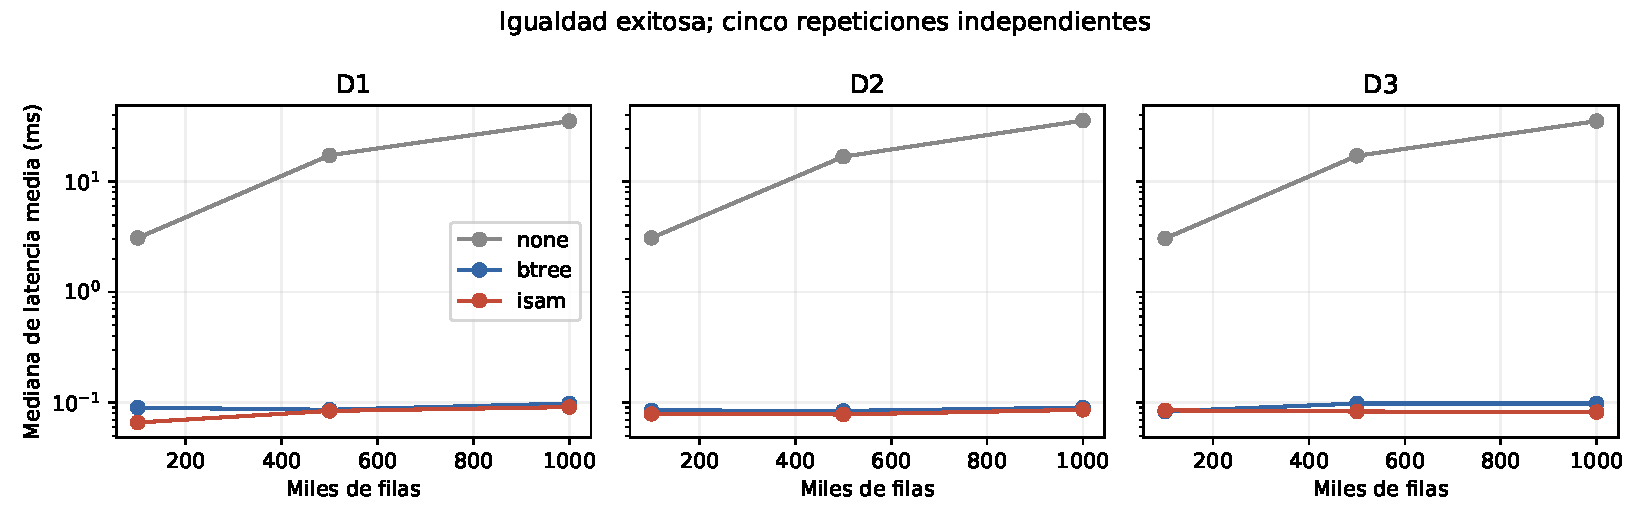
\includegraphics[width=\linewidth]{docs/results/figures/igualdad.pdf}\caption{Igualdad exitosa: escalabilidad observada bajo el protocolo registrado.}\end{figure}

\begin{figure}[htbp]\centering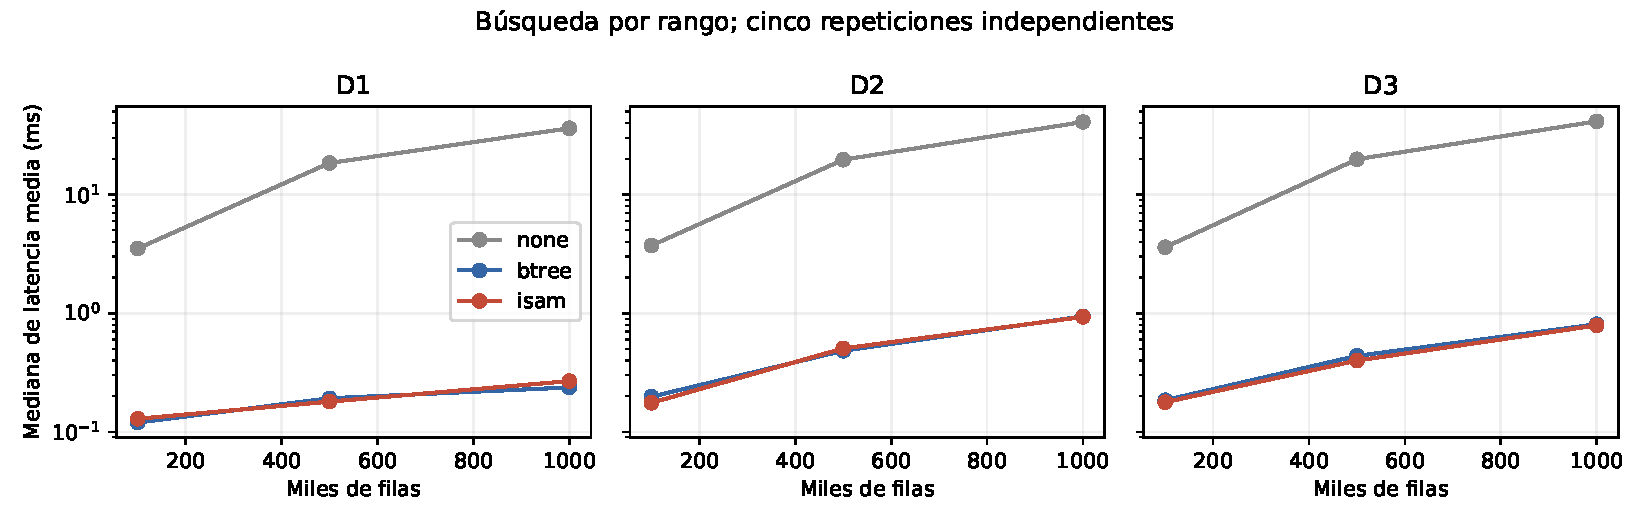
\includegraphics[width=\linewidth]{docs/results/figures/rango.pdf}\caption{Búsqueda por rango: escalabilidad observada bajo el protocolo registrado.}\end{figure}
